\chapter{Calcul par intervalle: éléments de base}

Le calcul par intervalle est décrit au départ dans les travaux de Ramon Moore \cite{Moore66}. L'utilité de ce mode de calcul vient des problèmes que représente le stockage des nombres réels dans nos ordinateurs via la norme \texttt{IEEE 754}. En effet, on sait avec cette norme facilement représenter une certaine quantité, finie de nombres réels tels que $0.5$, sous la forme $\text{signe} \times \text{base}^{exposant} \times (1 + mantisse)$. Il est en revanche impossible de représenter le reste des nombres réels, tels que $0.1$. De ce fait, lorsqu'on se place dans des contextes de calculs, il devient évident qu'on peut se retrouver à accumuler des erreurs de précision qui vont venir fausser les résultats. Quand on veut garantir des résultats, par exemple sur des problèmes d'optimisation, cela peut devenir pénalisant.

\section{Les intervalles}
\subsection{Intervalle et boite}

\begin{definition}
  On définit un \textit{intervalle} $[\underline{x}, \overline{x}]$ comme l'ensemble des nombres réels $x$ tels que $\underline{x} \leq x \leq \overline{x}$.
\end{definition}

On note par la suite plus généralement $[x] = [\underline{x}, \overline{x}]$.

\begin{ex}
  Si on veut représenter le nombre $\sqrt{2} = 1.4142\dots$, on peut dire: $1.4 \leq sqrt(2) \leq 1.5$, donc encadrer ce nombre par l'intervalle $[1.4, 1.5]$.
\end{ex}

\subsection{Fonctions d'inclusion}
% Fonction d'inclusion naturelle
Avec cette notion d'intervalle, on peut définir le comportement quand on applique une fonction. L'idée est de se dire que, pour un intervalle d'entrée $[x]$, l'intervalle image par une fonction $f$ doit contenir l'ensemble des images prises par la fonction $f$ pour tout les $x \in [x]$ :

\begin{definition}
    Soit $f : \mathbb{R}^n \rightarrow \mathbb{R}^m$ une fonction, la fonction $[f] : \mathbb{R}^n \rightarrow \mathbb{R}^m$ est une \textbf{fonction d'inclusion} pour $f$ si

    \begin{align}
        \forall[x] \in \mathbb{R}^n , f([x]) \subset [f]([x])
    \end{align}
\end{definition}

\begin{ex}
  La figure \ref{fig:fct2} montre l'encadrement d'une fonction $y = f(x)$ quelconque. La boite bleue est le produit cartésien de $[x]$ et de $[y]$.

  \begin{figure}[H]
    \centering
    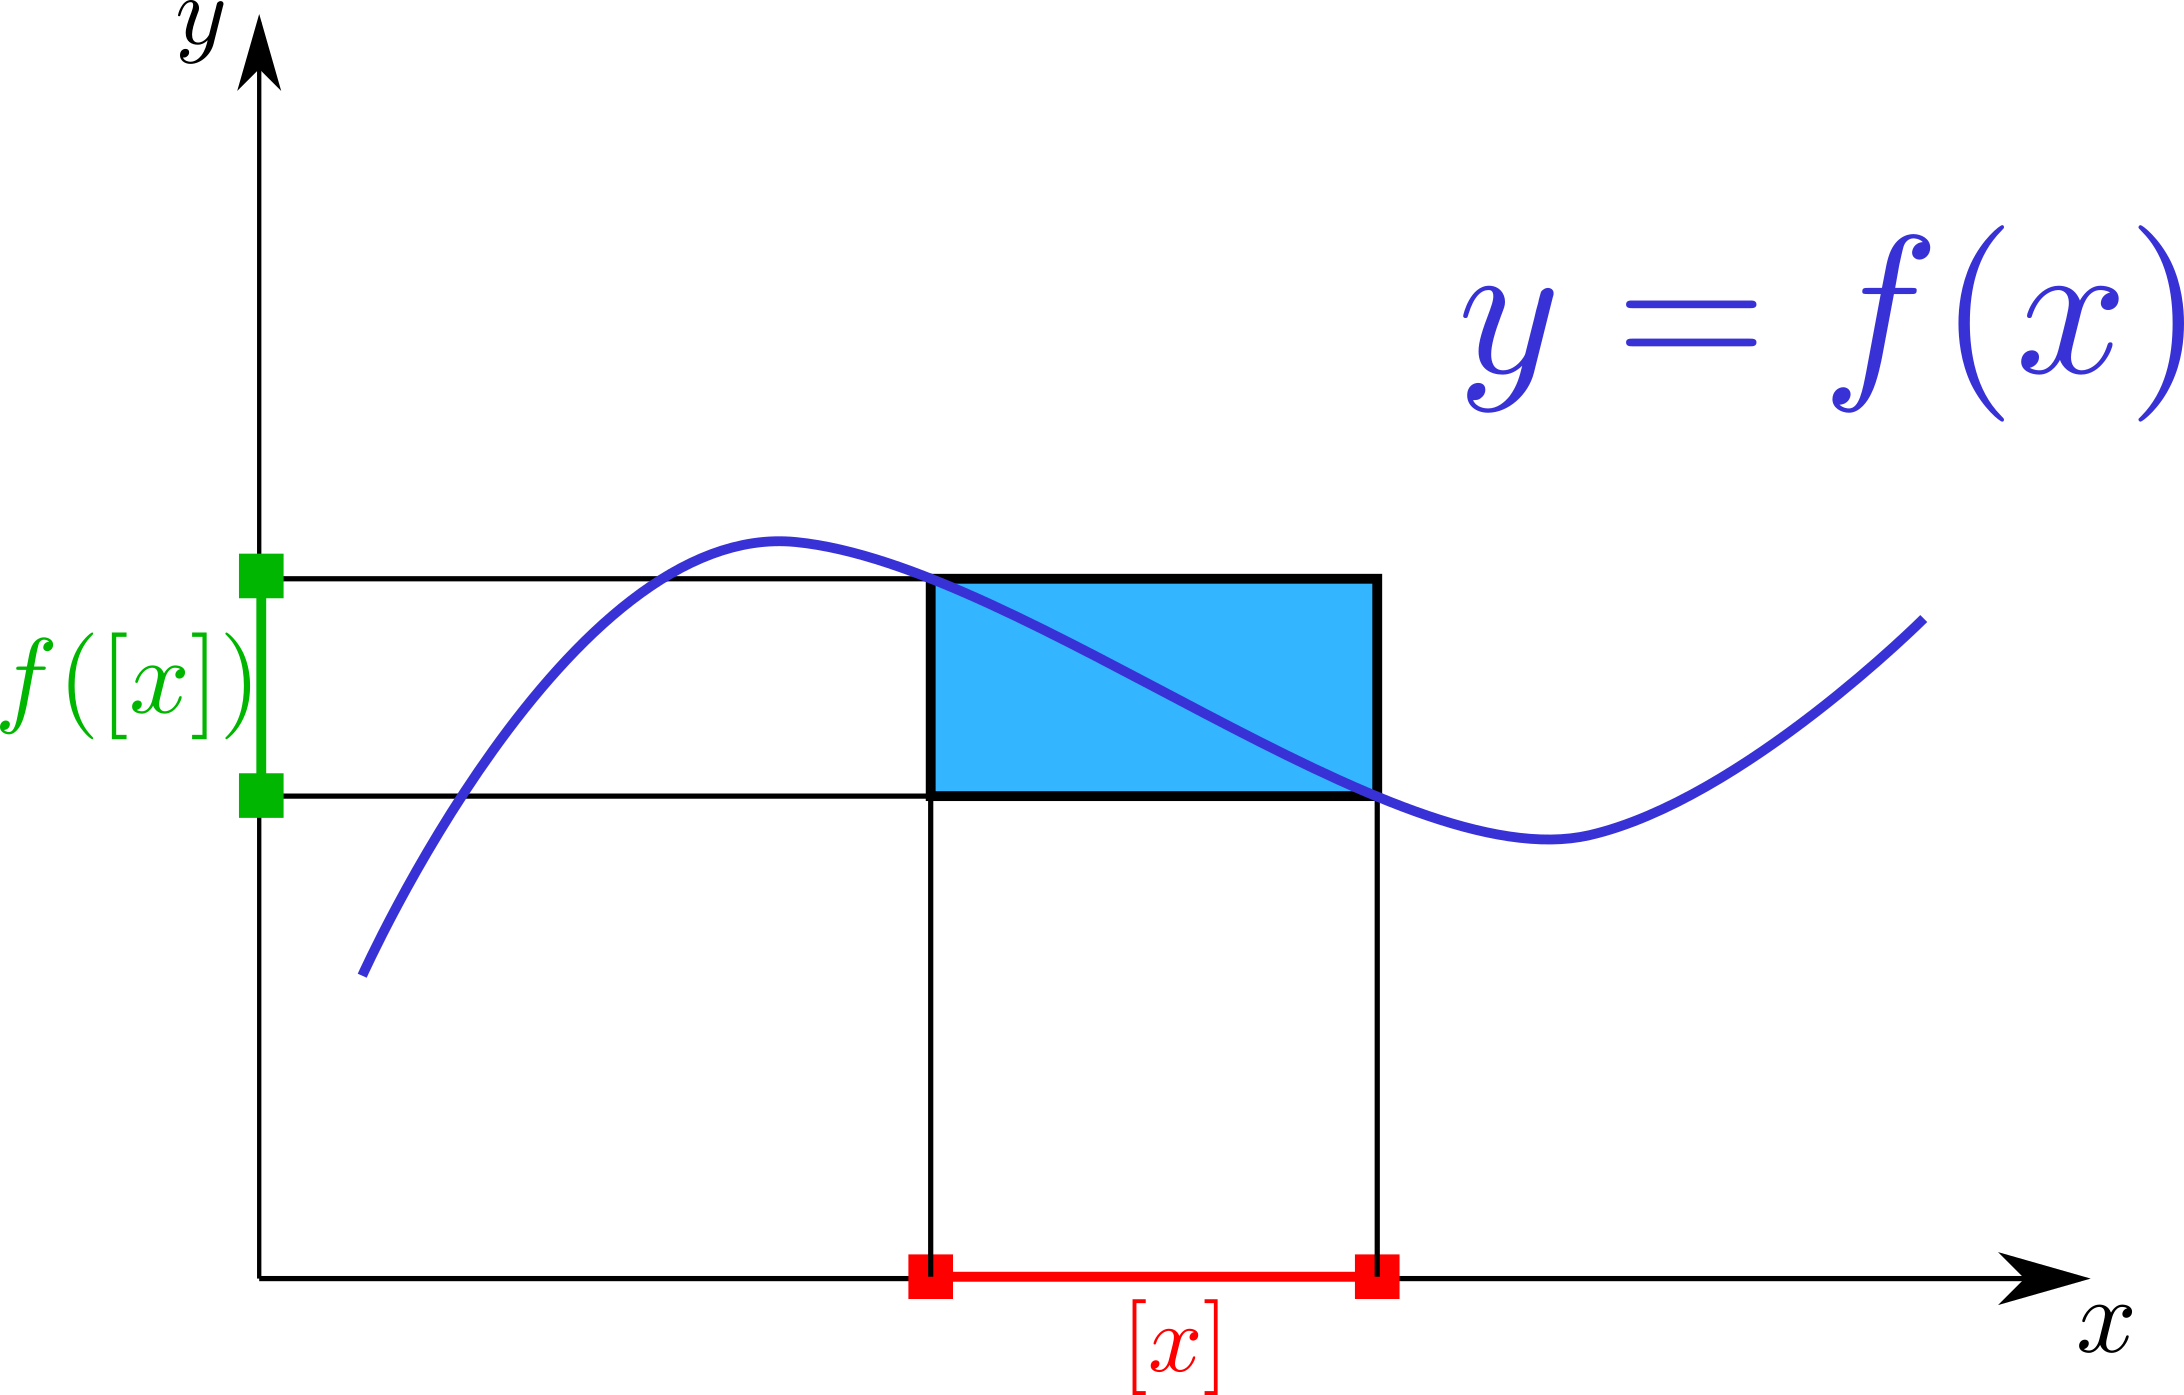
\includegraphics[scale=0.5]{intervaleval/function_eval_2.png}
    \caption{Fonction d'inclusion}
    \label{fig:fct2}
  \end{figure}
\end{ex}

L'encadrement nécessite la connaissance précise de la forme de la fonction pour pouvoir l'encadrer correctement. Ceci peut se révéler compliquer pour des fonctions non évidentes, typiquement quand on monte en dimension. Pour cela, on peut combiner les fonctions d'inclusion sans perdre la garantie d'inclusion, comme indiqué dans le théorème \ref{def:circ}.

\begin{theoreme}
  \label{def:circ}
  si $[f]$ et $[g]$ sont des fonctions d'inclusion respectives pour $f$ et $g$, alors $[f] \circ [g]$ est une fonction d'inclusion pour $f \circ g$.
\end{theoreme}

Cela permet en pratique de construire des fonctions d'inclusions élémentaires puis de les combiner. En effectuant cette opération, on peut en revanche perdre de la précision sur l'encadrement comme le montre la figure \ref{fig:fct3}.

\begin{figure}[H]
  \centering
  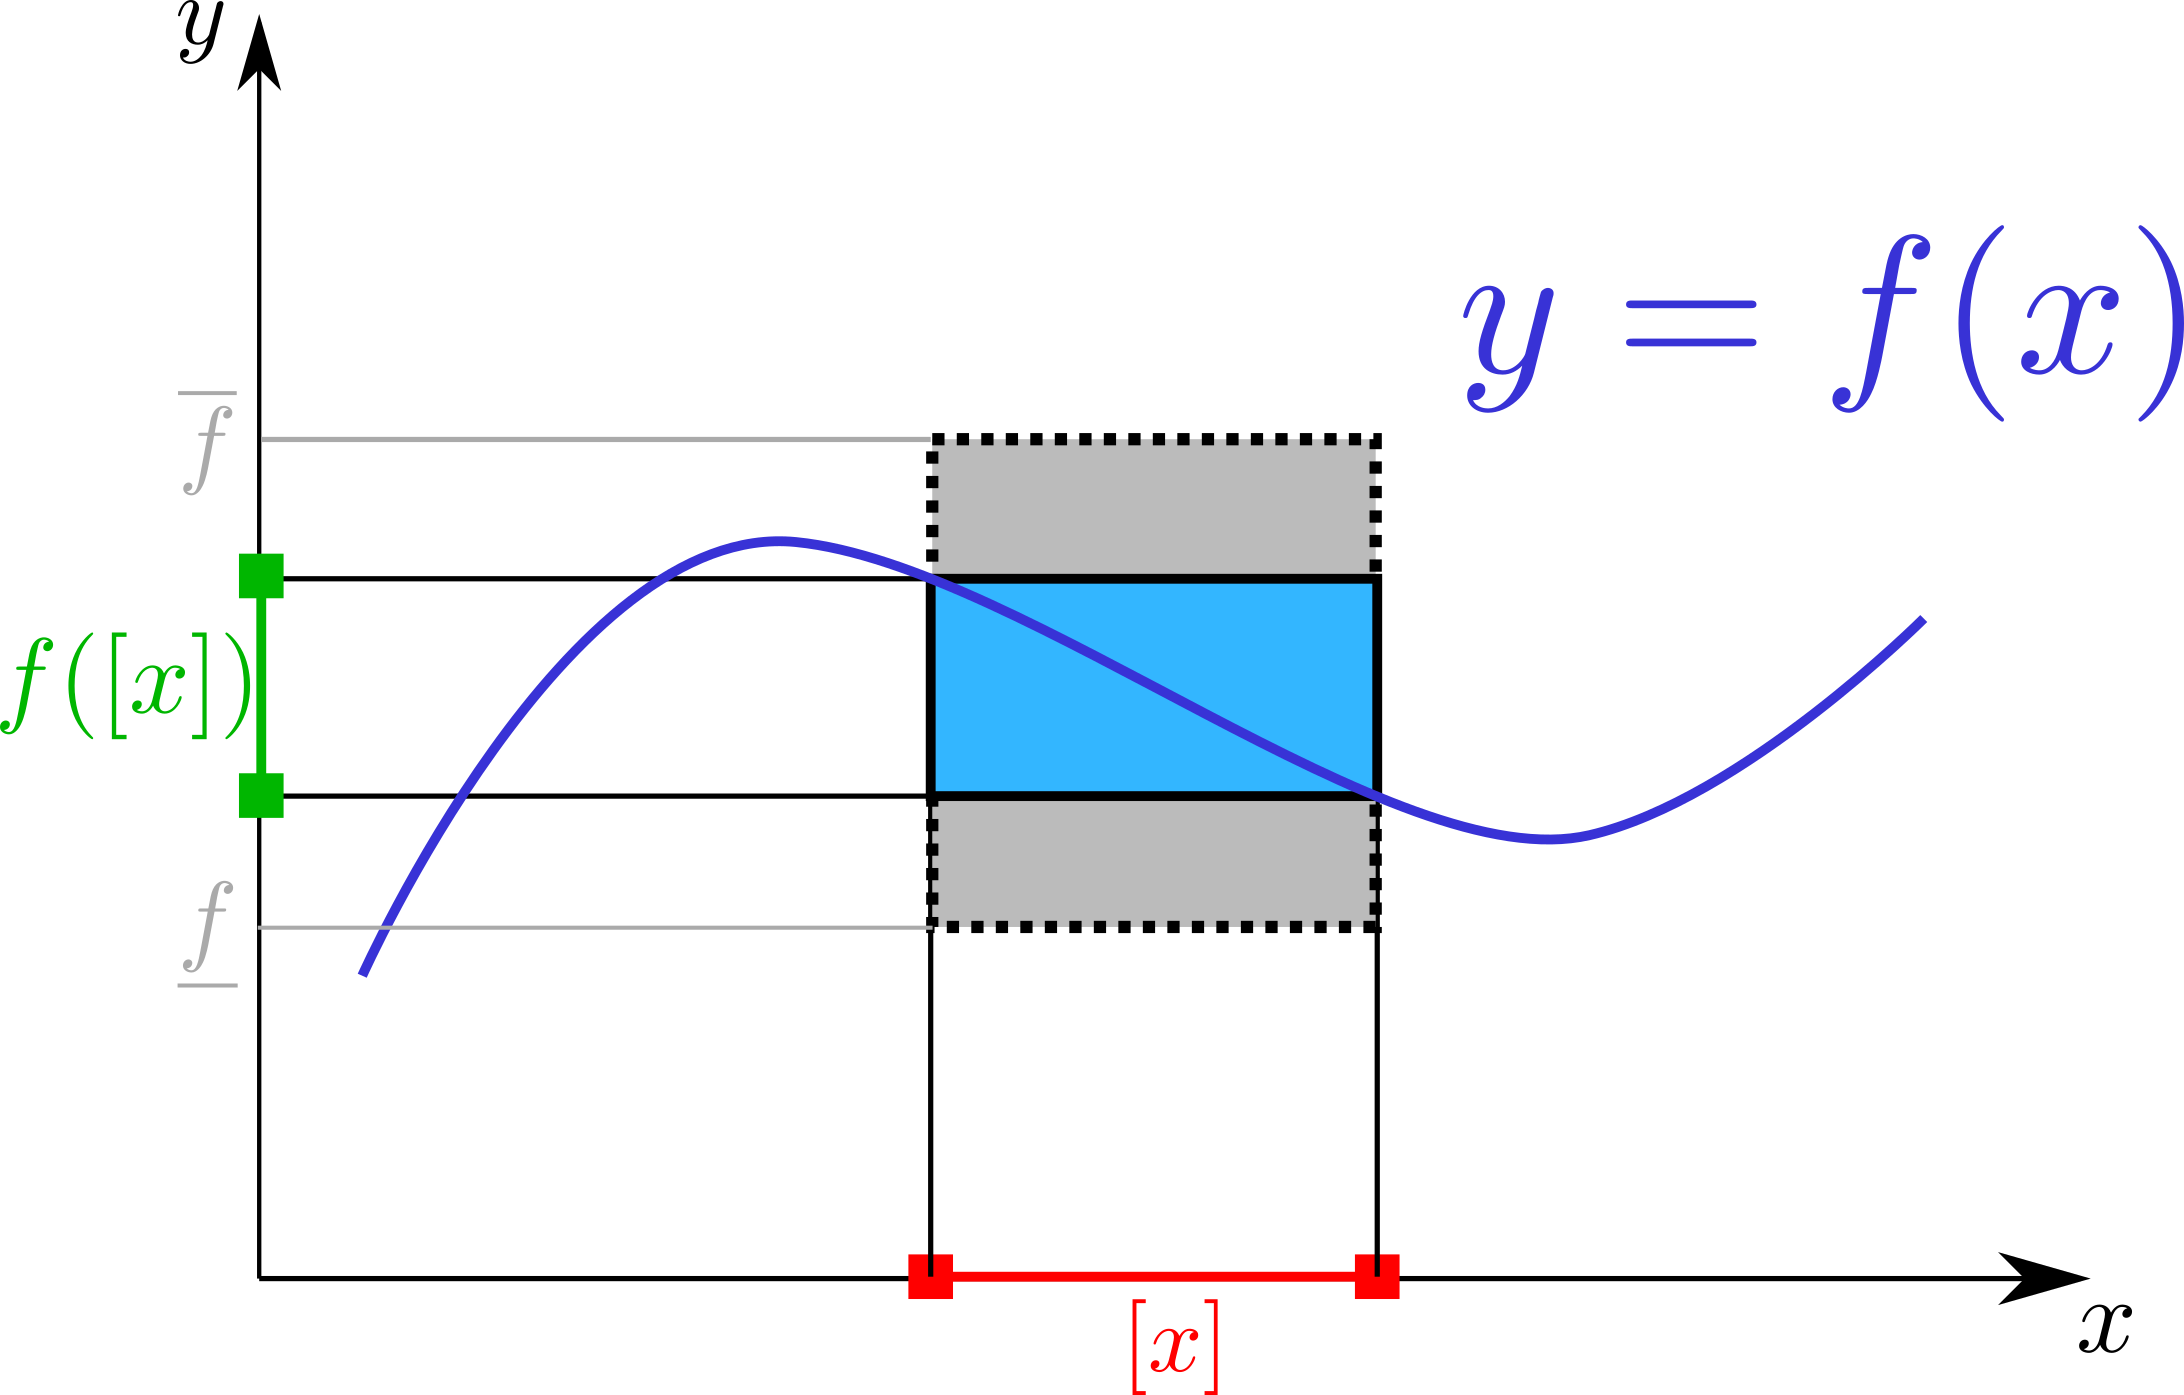
\includegraphics[scale=0.5]{intervaleval/function_eval_3.png}
  \caption{Fonction d'inclusion composée de moindre qualité}
  \label{fig:fct3}
\end{figure}

% Fonction d'inclusion par la forme centrée

\subsection{Arithmétique élémentaire}

Comme dit précédement, on peut construire les fonctions d'inclusions des fonctions necessaires pour n'importe quel problème en calcul par intervalle. Spécifiquement, il est utile de définir un certain nombre de fonctions de base permettant de former les blocs de construction pour la formation de fonctions plus complexes. On peut ainsi définir les opérateurs binaires (l'addition, la soustraction, la multiplication, \dots) ainsi que les opérateurs unaires (l'exponentielle, la puissance, le sinus, \dots).

\begin{ex}
  
  Un certain nombre de fonctions arithmétiques élémentaires peuvent être formulées :
  \begin{itemize}
    \item $[x_1] + [x_2] = [\underline{x_1} + \underline{x_2}, \overline{x_1} + \overline{x_2}]$
    \item $[x_1] - [x_2] = [\underline{x_1} - \overline{x_2}, \overline{x_1} - \underline{x_2}]$
    \item $[x_1] \times [x_2] = [\text{min}(\underline{x_1}\underline{x_2}, \underline{x_1}\overline{x_2}, \overline{x_1}\underline{x_2}, \overline{x_1}\overline{x_2}), \text{max}(\underline{x_1}\underline{x_2}, \underline{x_1}\overline{x_2}, \overline{x_1}\underline{x_2}, \overline{x_1}\overline{x_2})]$
    \item $[x]^2 = [0, \text{max}(\underline{x}^2, \overline{x}^2)]$
    \item $e^{[x]} = [e^{\underline{x}}, e^{\overline{x}}]$
    \item \dots
  \end{itemize}
\end{ex}

On peut étendre ces définitions à l'ensemble des fonctions strictements monotones: il est évident de se dire que, si une fonction $f(x)$ est strictement croissante, alors $[f]([x]) = [f(\underline{x}), f(\overline{x})]$, et de même pour une fonction décroissante. On peut alors construire des fonctions plus complexes, comme $f : x \mapsto x^3$ en découpant la définition de la fonction par morceaux.

\section{Optimisation avec les intervalles}
On met en place un algorithme d'optimisation utilisant le calcul par intervalle pour obtenir un encadrement garanti de la solution à notre problème.

On veut résoudre le problème $\max(f(x))$ tel que $g(x) \leq 0$, avec $f$ fonction coût et $g$ ensemble des contraintes. Avec le calcul par intervalle, on cherche à avoir un encadrement \textit{garanti} de la solution au problème. Le principe de base est de découper l'ensemble des entrées en un certain nombre de boites, dépendant de la précision que l'on veut, comme à la figure \ref{fig:optim1}. On choisit ensuite un $a$ solution admissible du problème suivant le théorème \ref{thm:solutionsup}.

\begin{theoreme}
  \label{thm:solutionsup}
  Soit un $a$ une solution admissible du problème $\max\limits_{x} f(x)$ tel que $g(x) \leq 0$ et $x^*$ la solution optimale, on a:
  \begin{align}
      sup([f]([x])) \leq f(a) \Rightarrow x^* \notin [x]
  \end{align}
\end{theoreme}

\begin{figure}[H]
  \centering
  \begin{subfigure}[h]{0.3\textwidth}
      \centering
      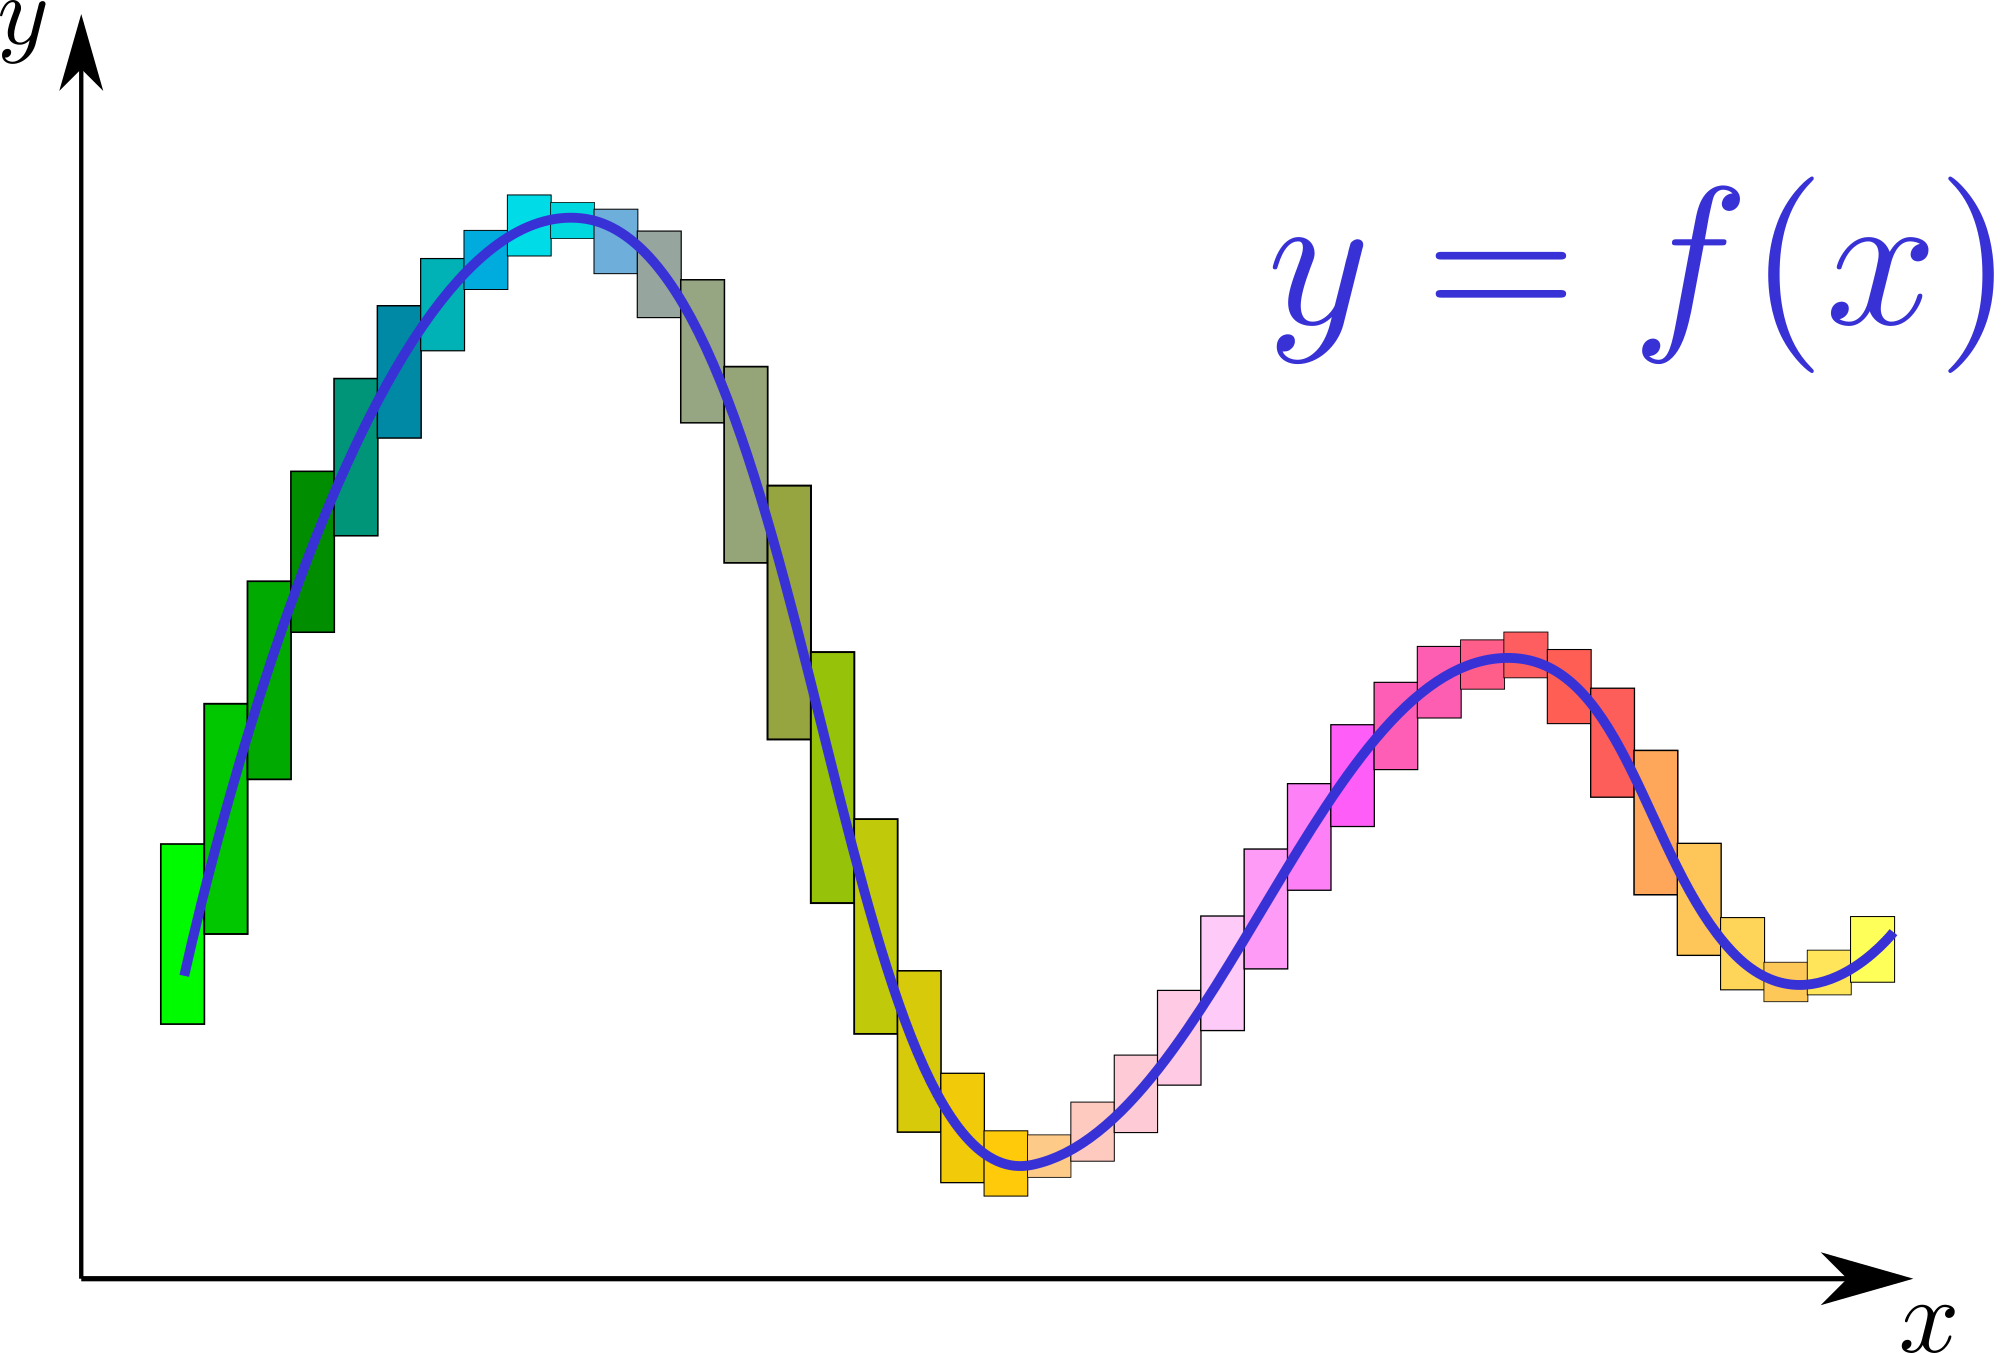
\includegraphics[scale=0.4]{AlgoOptim/function_optim_1.png}
      \caption{}
      \label{fig:optim1}
  \end{subfigure}
  \begin{subfigure}[h]{0.3\textwidth}
      \centering
      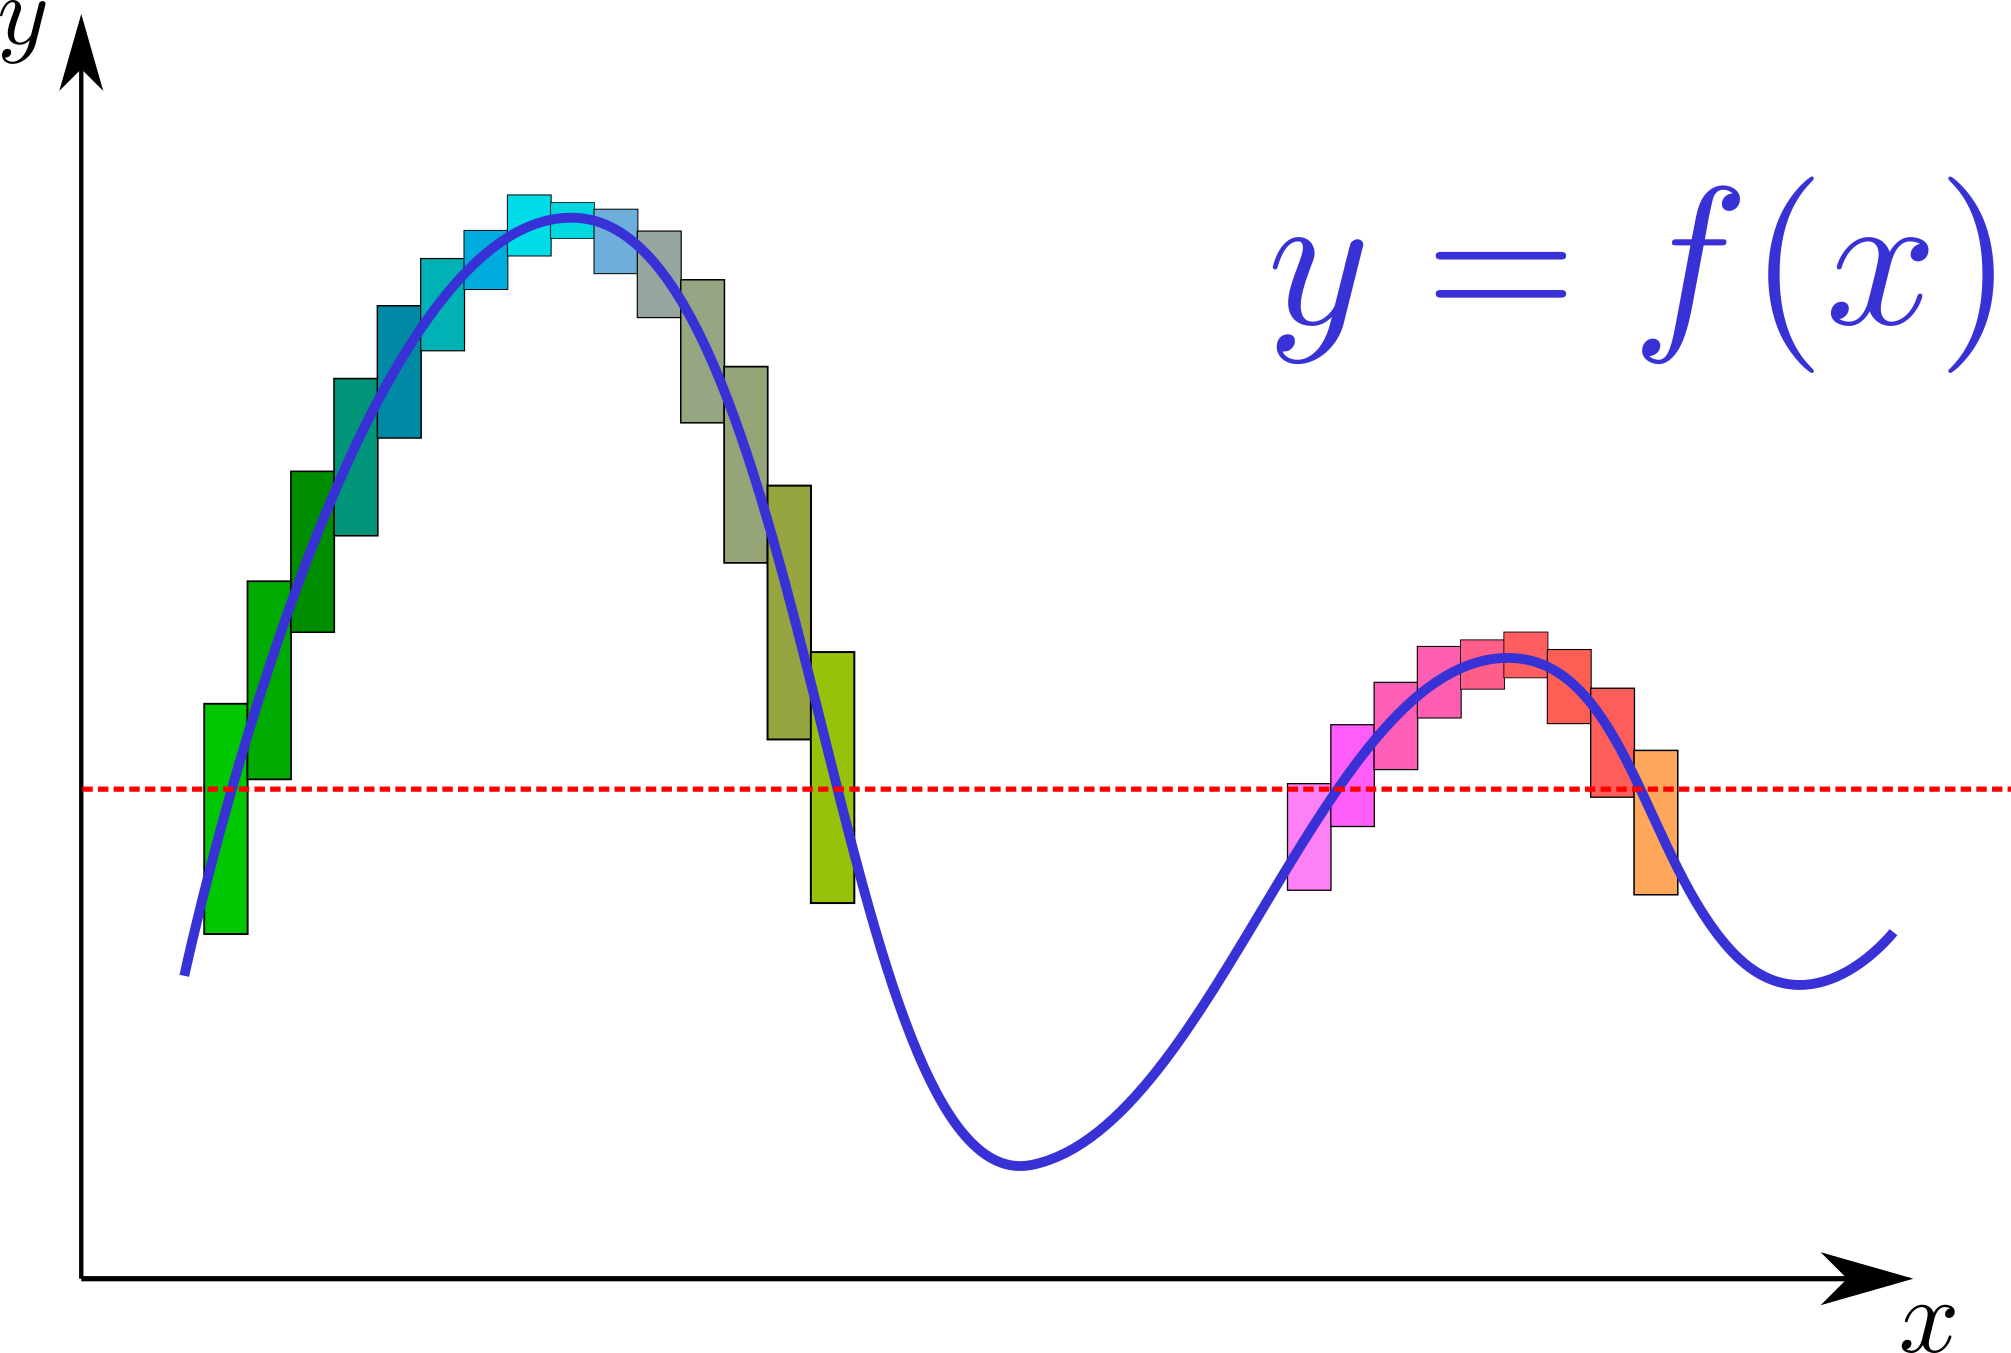
\includegraphics[scale=0.4]{AlgoOptim/function_optim_4.png}
      \caption{}
      \label{fig:optim2}
  \end{subfigure}
  \begin{subfigure}[h]{0.3\textwidth}
      \centering
      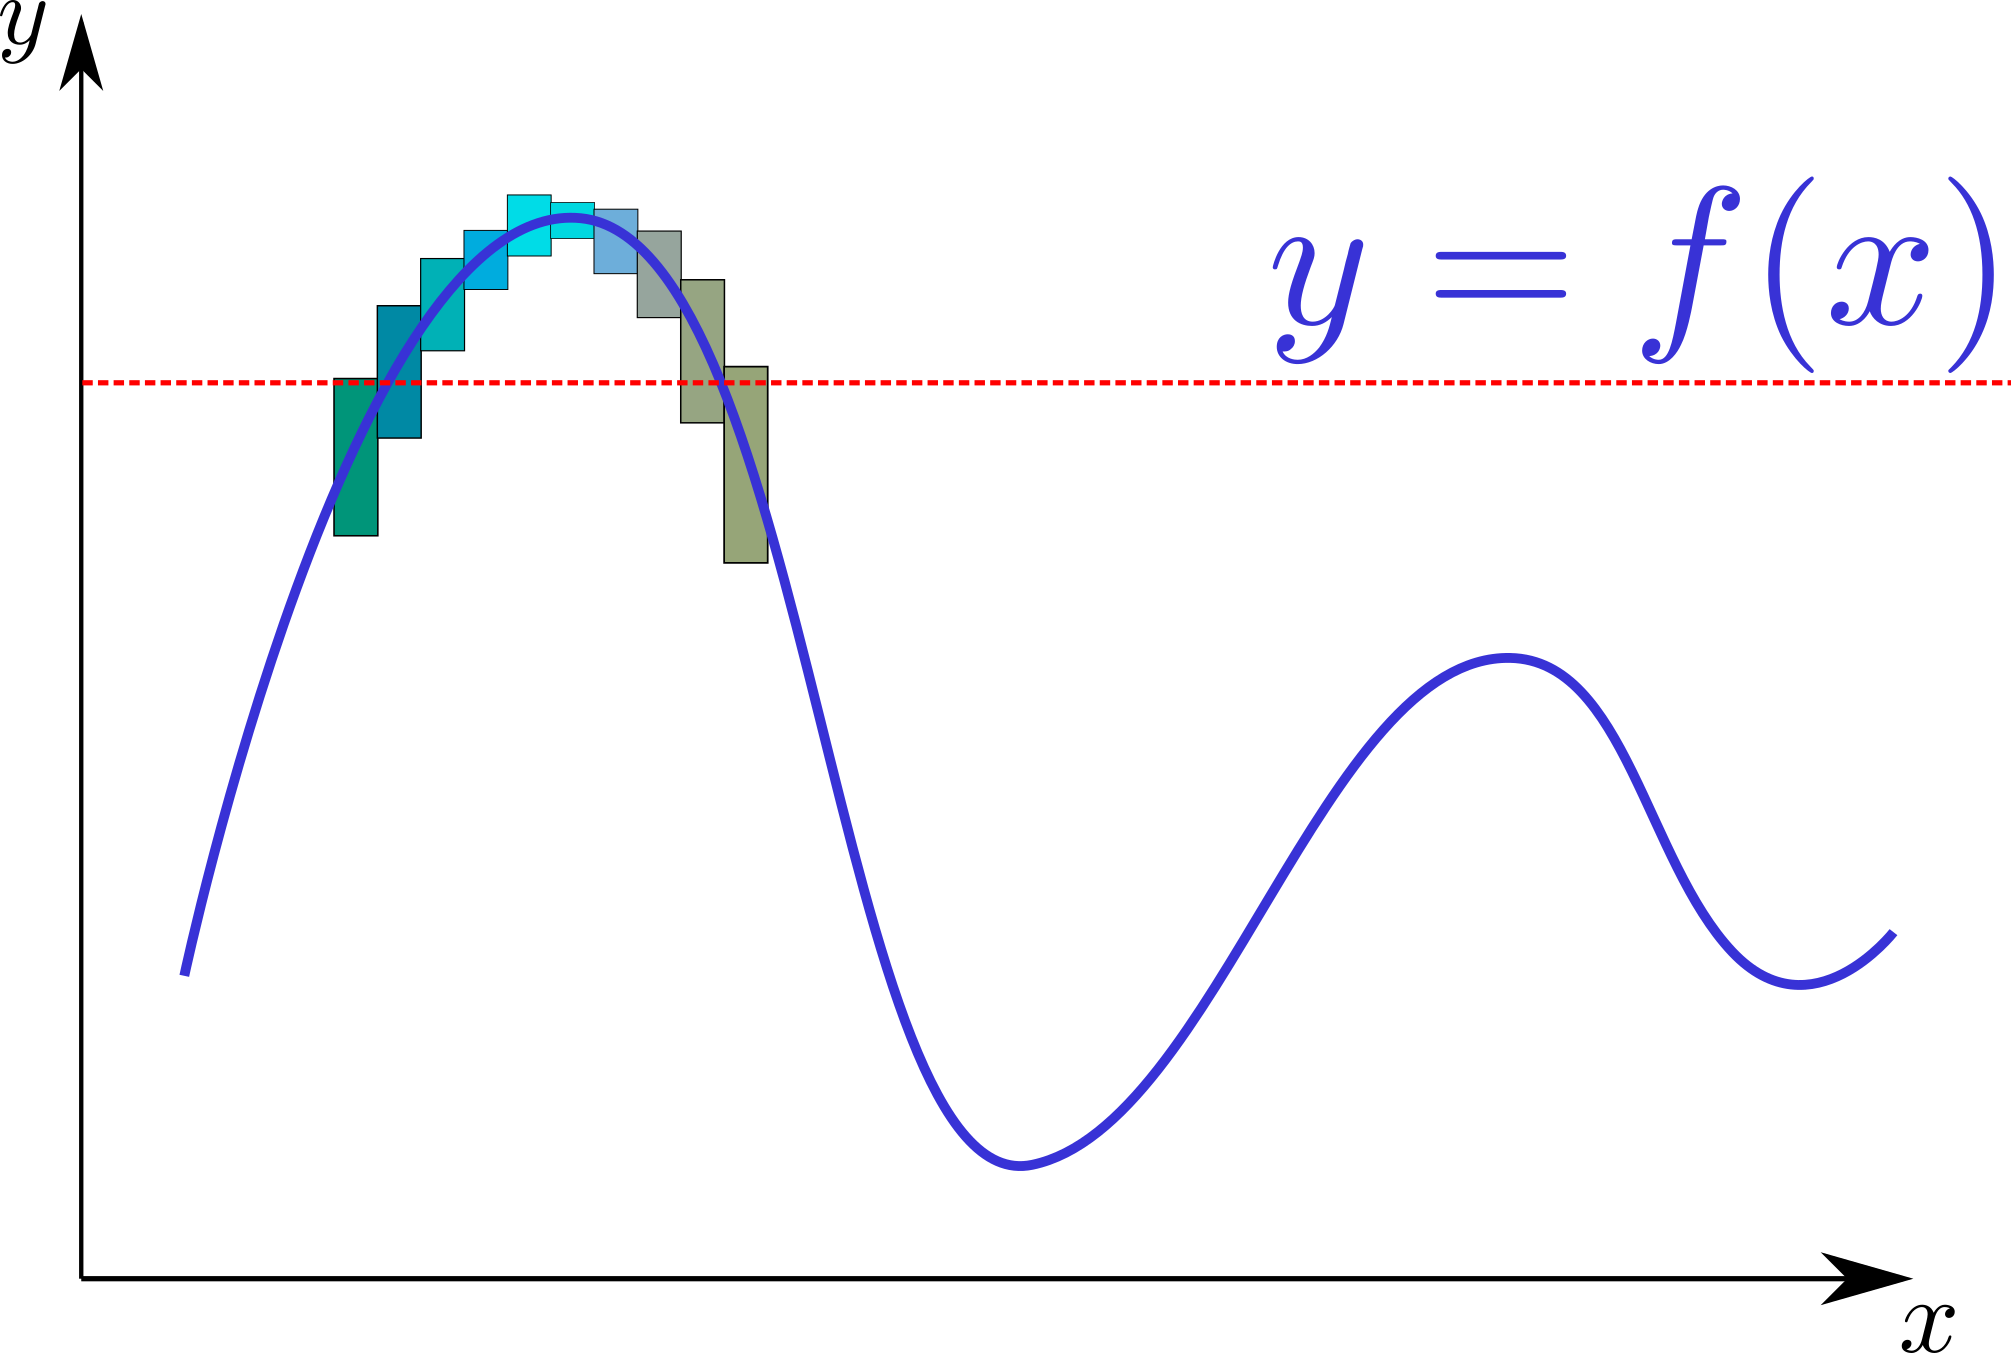
\includegraphics[scale=0.4]{AlgoOptim/function_optim_6.png}
      \caption{}
      \label{fig:optim3}
  \end{subfigure}
  \caption{Optimisation naïve}
\end{figure}


La figure \ref{fig:algomaxim} présente l'algorithme utilisé pour ce problème de maximisation (la logique étant la même pour une minimisation). Quatre éléments sont important à comprendre dans cet algorithme.

\begin{figure}[H]
    \begin{algorithm}[H]
        \SetAlgoLined
        \KwData{
          $[I_{init}]$ initial search box;
          $\epsilon$ stop criterion;
          $f$ cost function;
          $g$ constraints function;
        }
        \KwOut{
          $[f]$ bounds of best solution; $[I]$ solution box
        }
        \Begin{
          $\texttt{solutions}$ list of solution boxes\;
          Add $[I_{init}]$ to $\texttt{solutions}$\;
          $[f_{c}]$ current bounds of solutions\;
          \While{$\overline{f_{c}} - \underline{f_{c}} \geq \epsilon$}{
              $\texttt{currentSolutions}$ empty list of boxes\;
              \tcc{Bisect, evaluate cost, manage constraints}
              \ForAll{$\texttt{sol}$ in $\texttt{solutions}$}{
                    $[\texttt{left}], [\texttt{right}] \longleftarrow \texttt{bisect}(\texttt{sol})$\;
                    \If{$\texttt{g}([\texttt{left}])$ is valid}{
                        Add $[\texttt{left}]$ to $\texttt{currentSolutions}$\;
                    }
                    \If{$\texttt{g}([\texttt{right}])$ is valid}{
                        Add $[\texttt{right}]$ to $\texttt{currentSolutions}$\;
                    }
              }
              \tcc{Remove boxes certified not to contain maximum}
              Evaluate $[f]$ for all $[\texttt{currentSolutions}]$\;
              $f_{best}$ best $f(\texttt{sol}.\texttt{mid})$ in all $[f]$ \;
              Remove all $[\texttt{sol}]$ in $[\texttt{currentSolutions}]$ where $sup([f]([sol])) \leq f_{best}$\;
              $\texttt{solutions} \longleftarrow \texttt{currentSolutions}$
          }
          \Return{$\texttt{solutions}, [f_{c}]$}
        }
      \end{algorithm}

    \caption{Algorithme de maximisation par le calcul par intervalle}
    \label{fig:algomaxim}
\end{figure}


